\section{Level surfaces}
                In the planar case, we would often have to specify a set of points like
                \[
                x^2+y^2=1
                \]
                which is the circle.  
                
                In higher dimensions, we can do the same in order to visualize functions of the form $f\colon \R^3\to \R$ written as $f(x,y,z)$.  If we pick some constant $c$ and write
                \[
                f(x,y,z)=c
                \]
                then we will get the \textbf{level surfaces} for the function $f(x,y,z)$.  Visualizing functions of three variables (or more) $f(x,y,z)$ requires us to visualize in four or more dimensions. So we often reduce the problem to visualizing level surfaces.
                
                \begin{ex}{A Sphere as a Level Surface}{sphere_lev_surf}
                We can consider the following function
                \[
                f(x,y,z)=x^2+y^2+z^2.
                \]
                If we take the one level set, that is the points $(x,y,z)$ that satisfy
                \[
                x^2+y^2+z^2=1
                \]
                then we get the \emph{2-sphere}.  These are the set of points that are all a distance one from the origin.  Here is a picture:
                \begin{figure}[H]
                    \centering
                    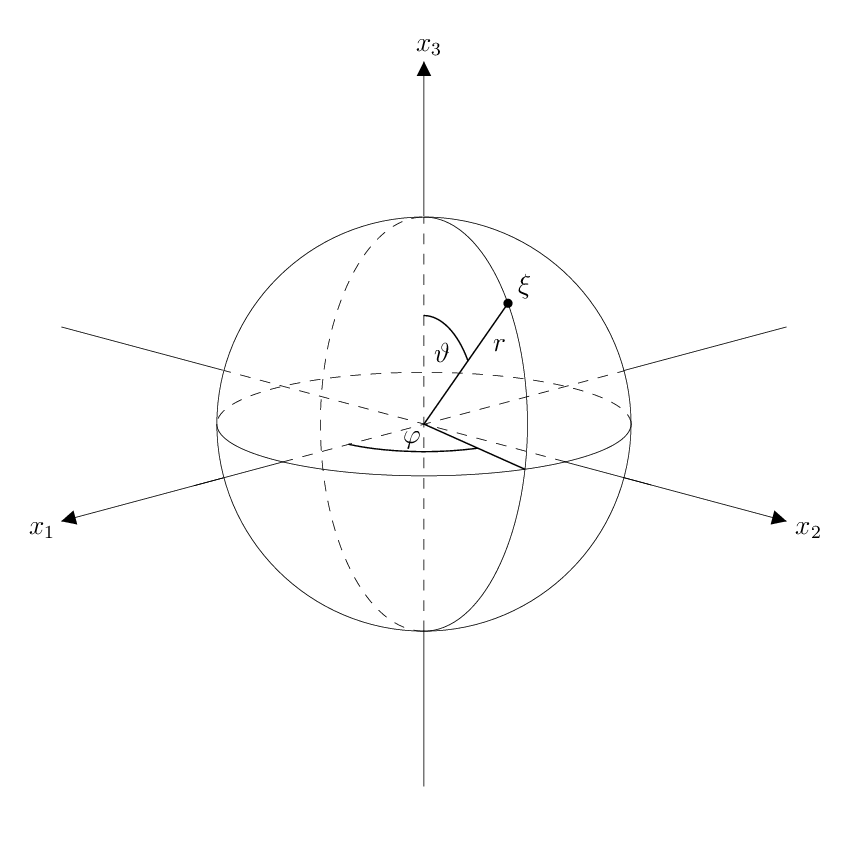
\includegraphics[width=.4\textwidth]{Figures_Part_6/sphere.png}
                \end{figure}
                \end{ex}
                
                \begin{ex}{The Hyperboloids}{hyperboloids}
                Consider a family of surfaces given by the level surfaces of
                \[
                f(x,y,z)=x^2+y^2-z^2.
                \]
                \begin{itemize}
                    \item If we take $c=0$ and set
                    \[
                    x^2+y^2-z^2=0.
                    \]
                    then we find the 0 level surface. In this case, we can do a bit of work to find
                    \[
                    z=\pm \sqrt{x^2+y^2}.
                    \]
                    Notice, if we pick any value for $z$, that we get a circle at that level!  When $z=0$, we get a single point.  It turns out that we get the \emph{(double) cone} surface which looks like
                    \begin{figure}[H]
                        \centering
                     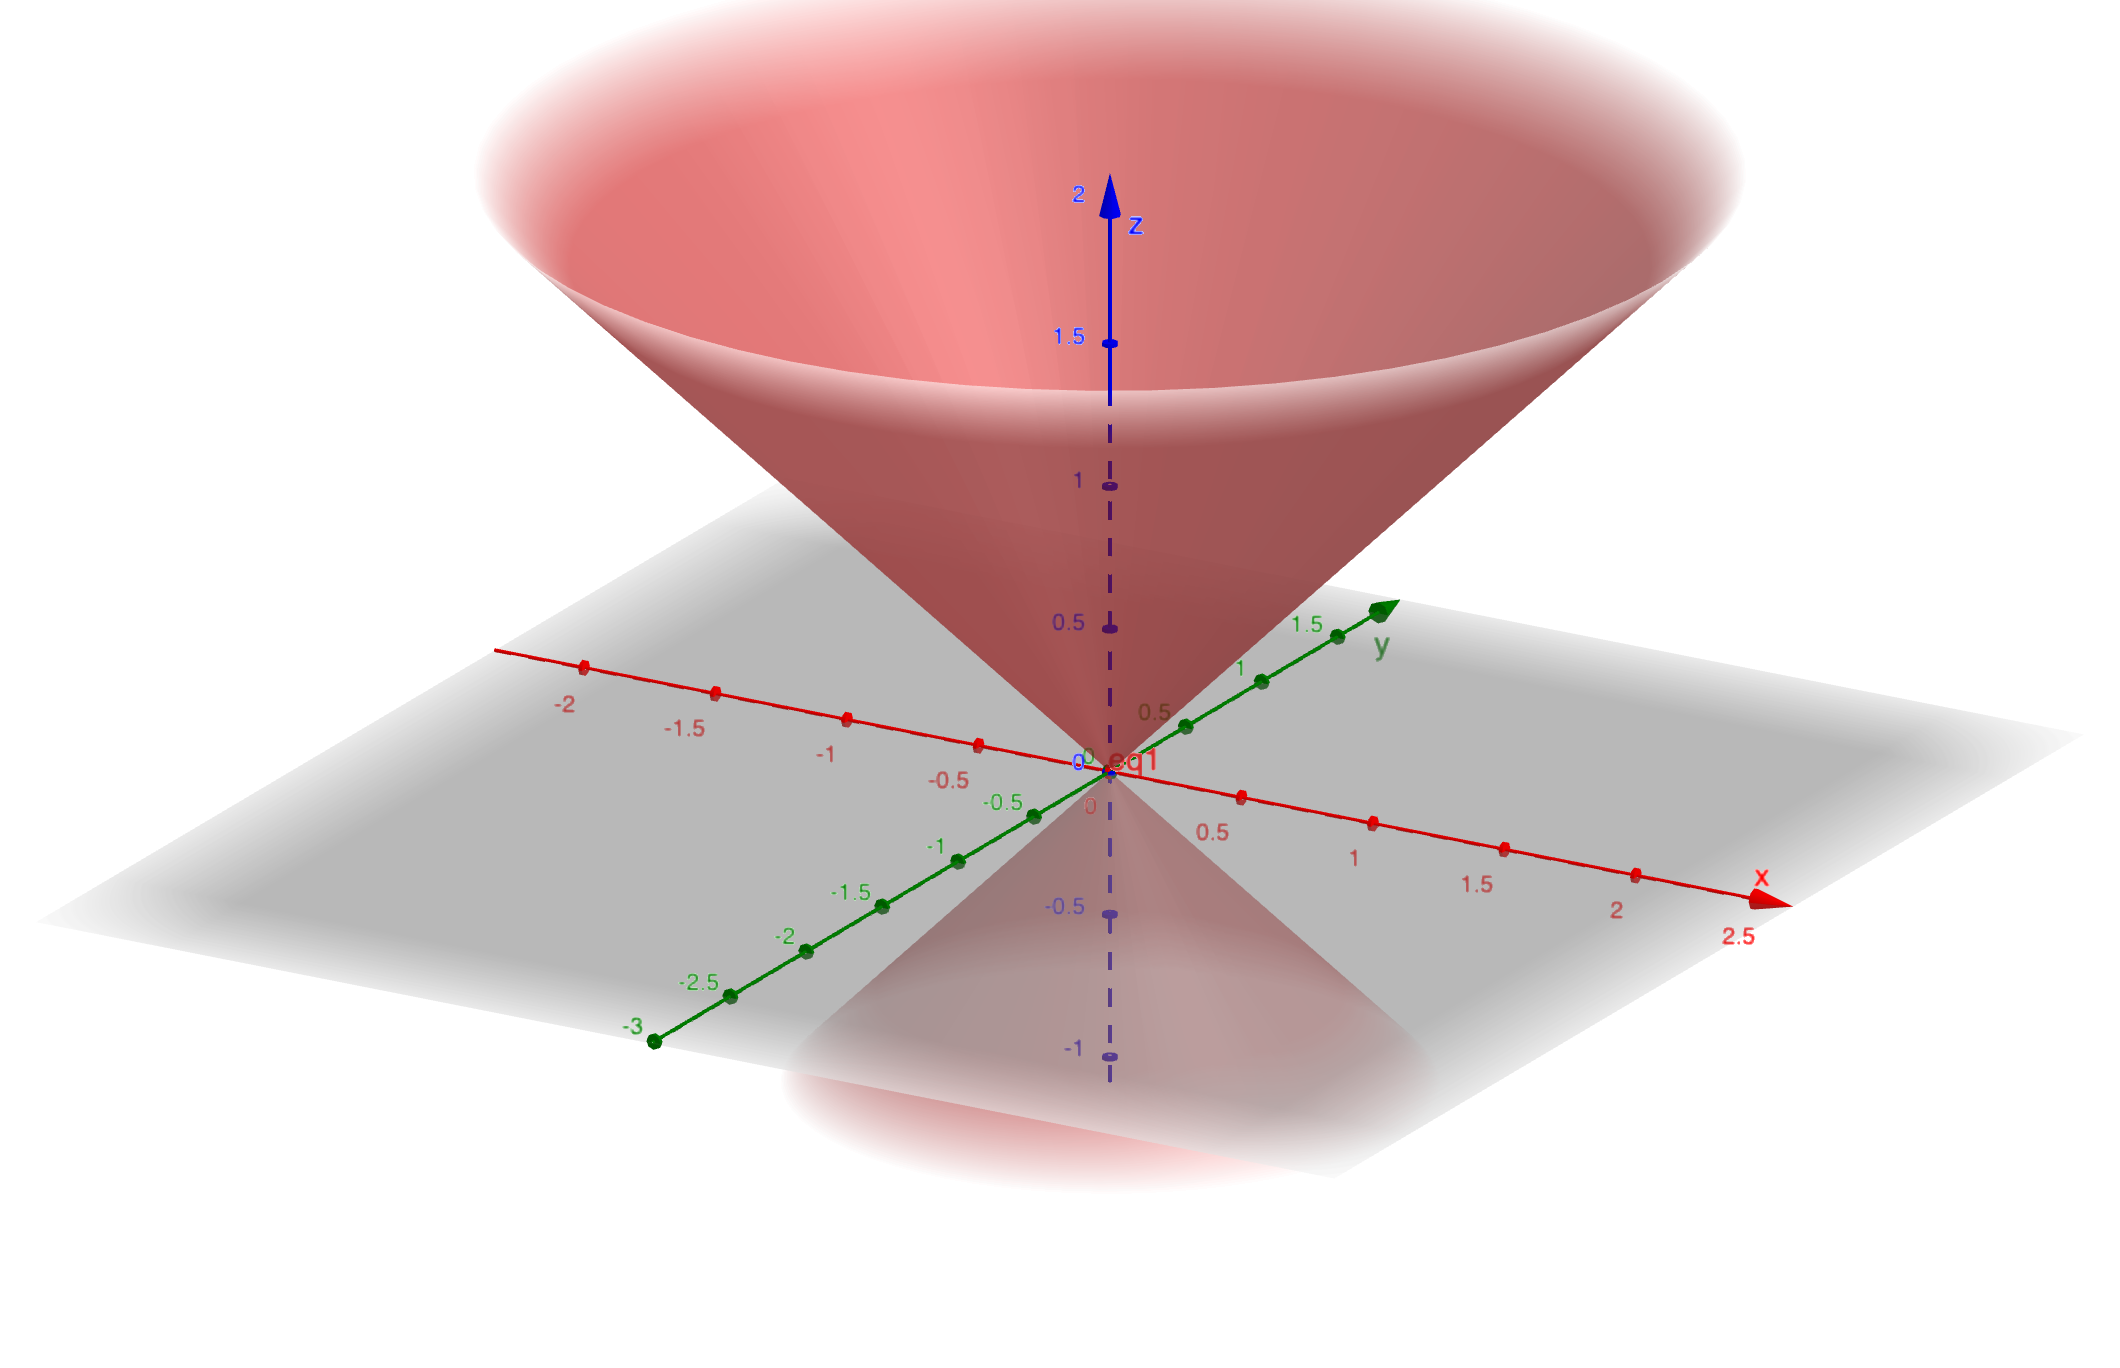
\includegraphics[width=.4\textwidth]{Figures_Part_6/cone_surface.png}
                    \end{figure}
                    
                    \item If we take $c=1$ and set
                    \[
                    x^2+y^2-z^2=1
                    \]
                    we get the \emph{hyperboloid of one sheet}.  This looks like
                    \begin{figure}[H]
                        \centering
                        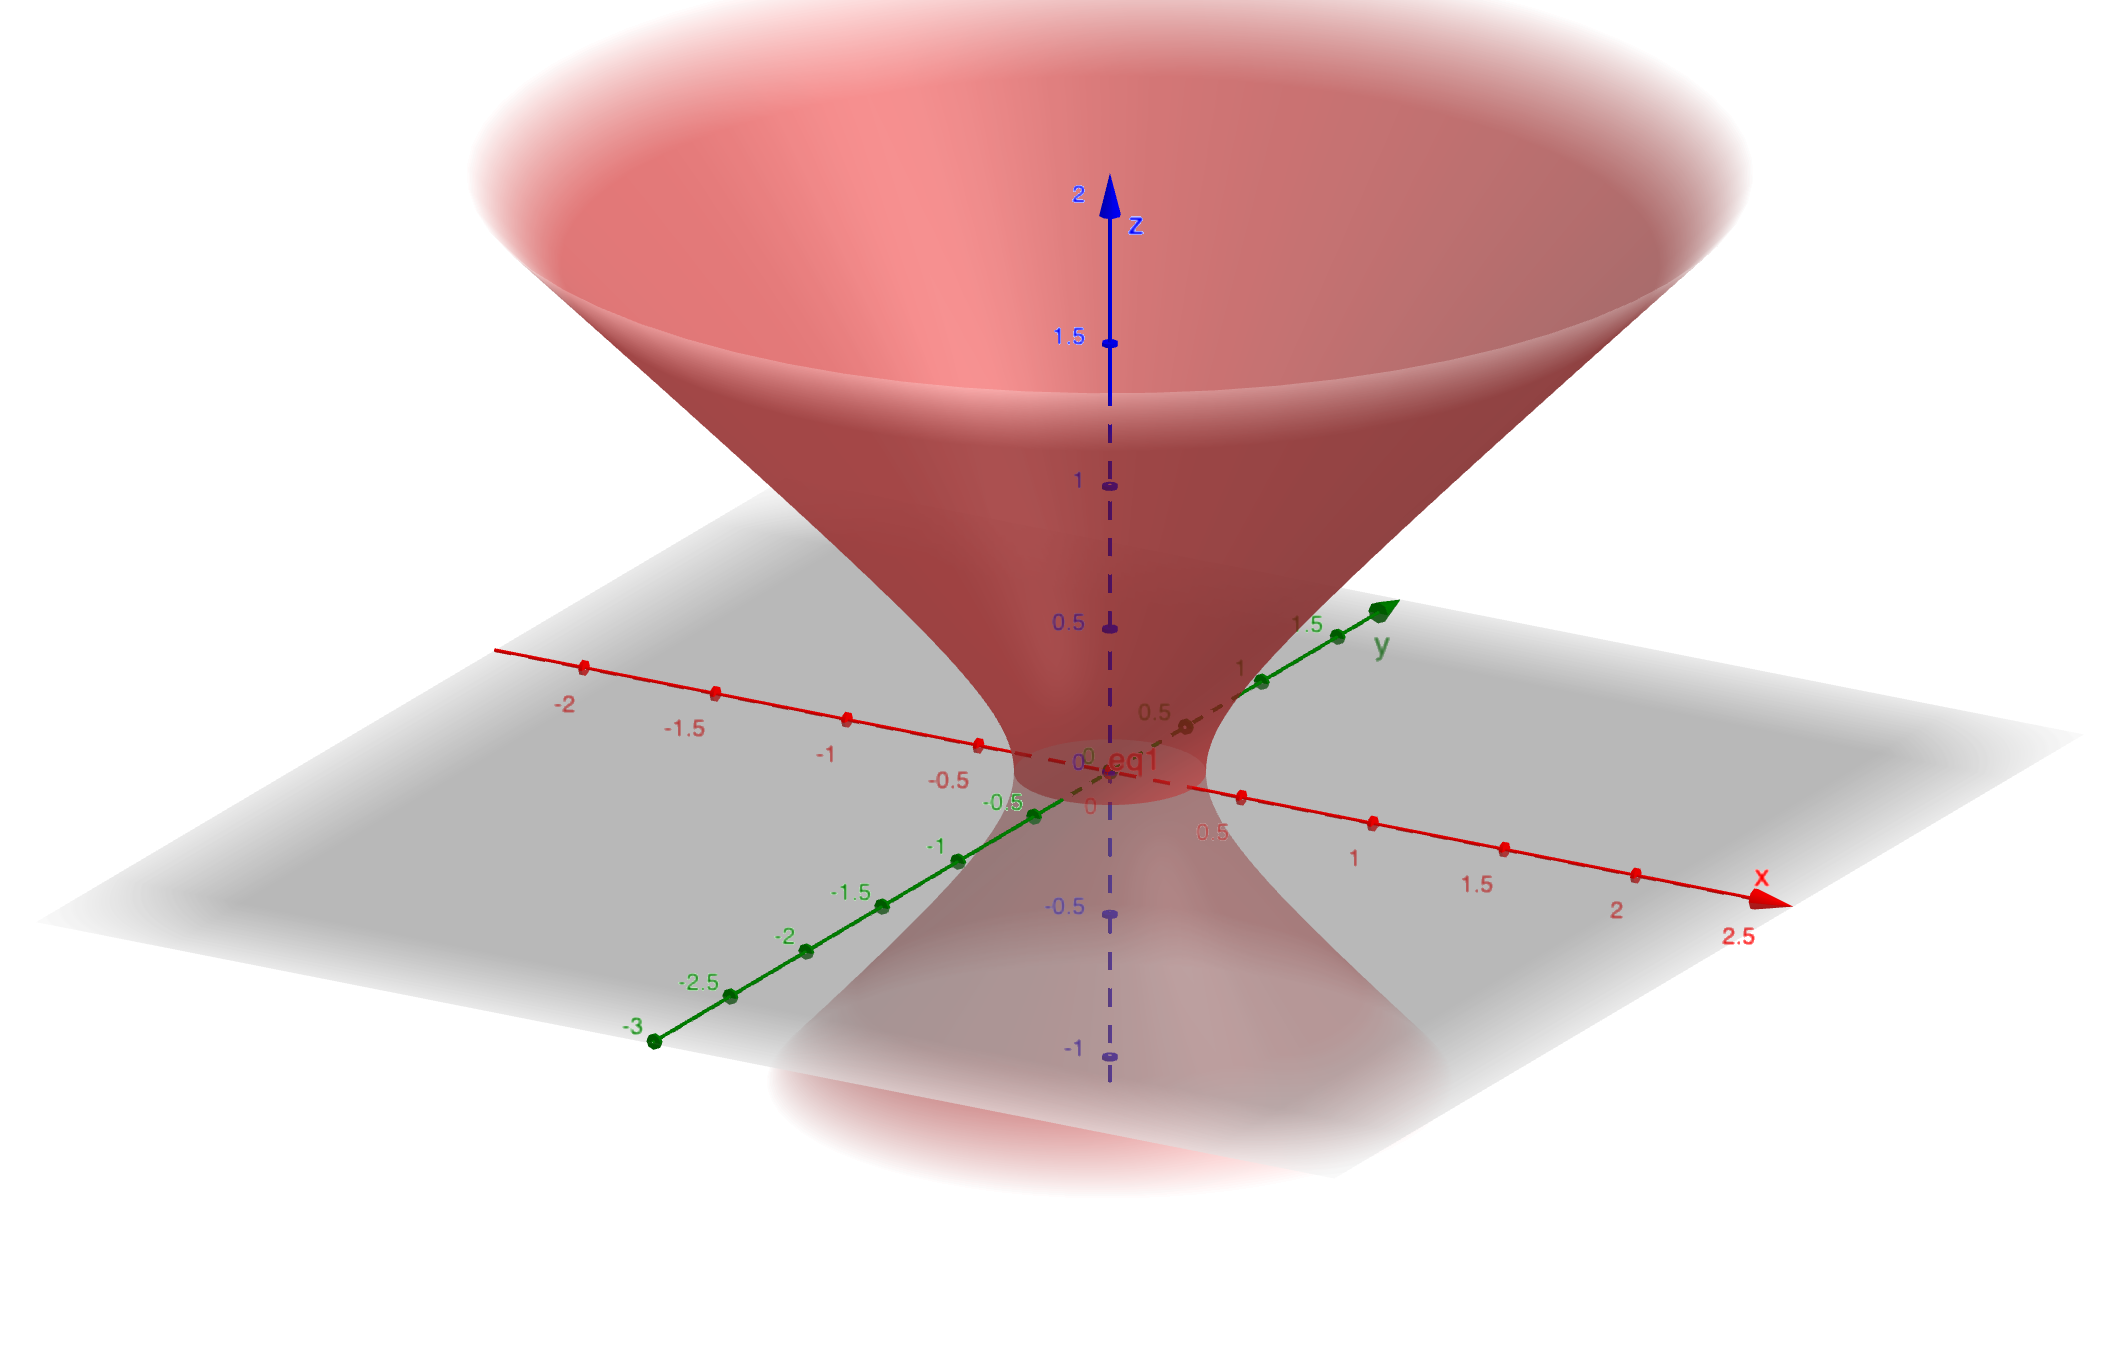
\includegraphics[width=.4\textwidth]{Figures_Part_6/hyperboloid_1_sheet.png}
                    \end{figure}
                    
                    \item If we take $c=-1$ and set
                    \[
                    x^2+y^2-z^2=-1
                    \]
                    we get the \emph{hyperboloid of two sheets}.  This looks like
                    \begin{figure}[H]
                        \centering
                        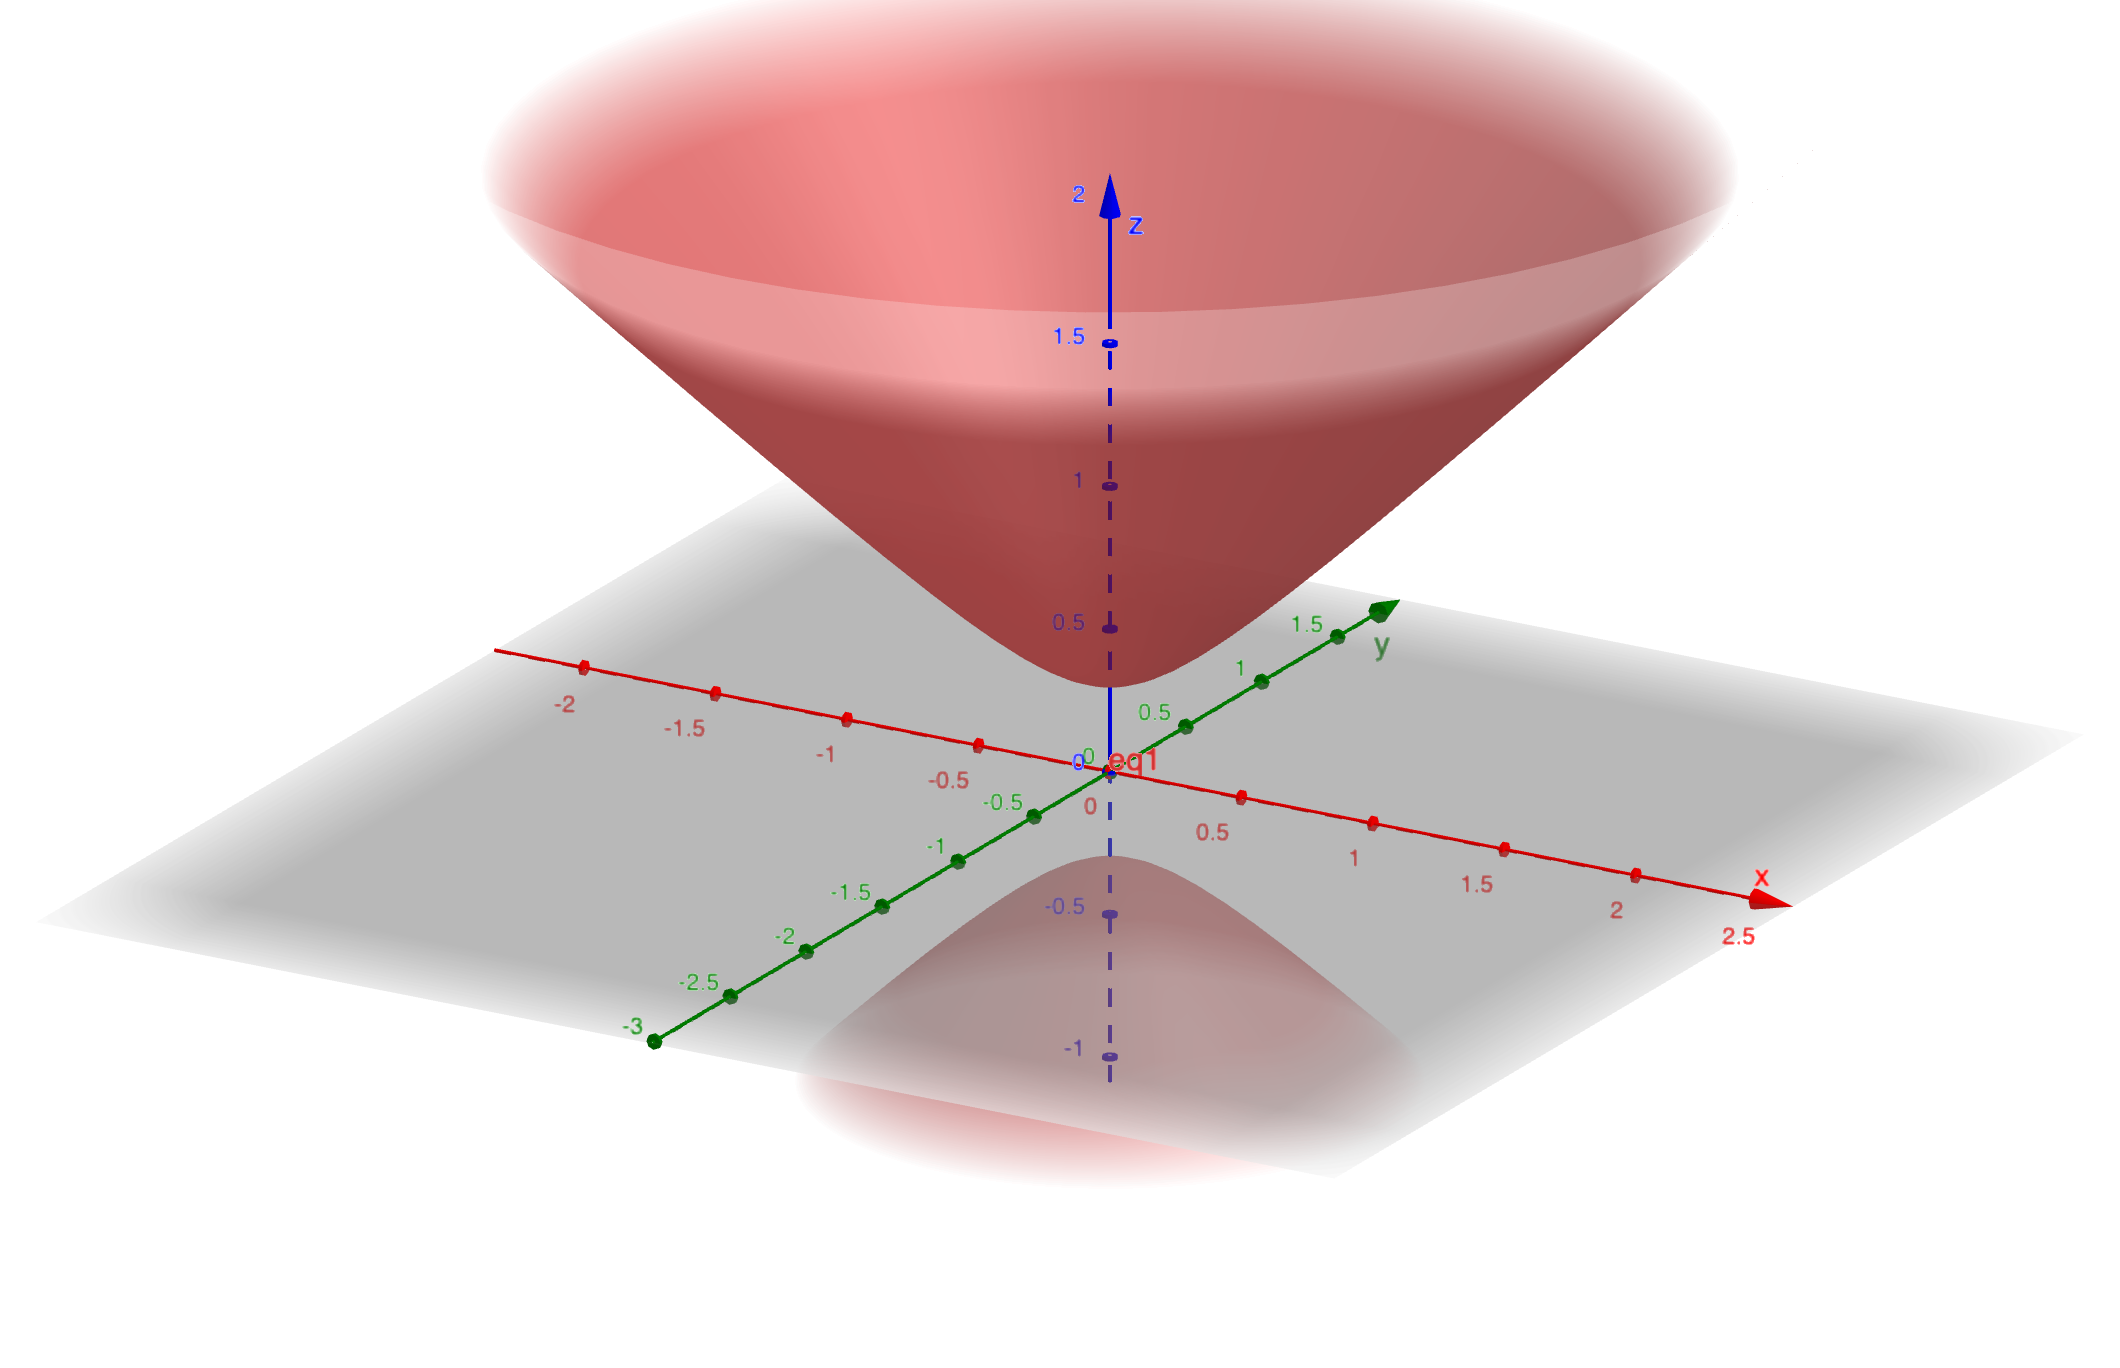
\includegraphics[width=.4\textwidth]{Figures_Part_6/hyperboloid_2_sheet.png}
                    \end{figure}
                \end{itemize}
                \end{ex}
                
                \begin{ex}{The Torus}{torus}
                For this example, I will choose specific nice numbers, but this is a yet another case of a level surface.  Take
                \[
                \left(5-\sqrt{x^2+y^2}\right)^2+z^2=2.
                \]
                This gives us the \emph{torus} with inner radius (the radius from the center of the donut hole to the center of the tube) $5=R$ and tube radius $2=r$. This looks like
                \begin{figure}[H]
                    \centering
                    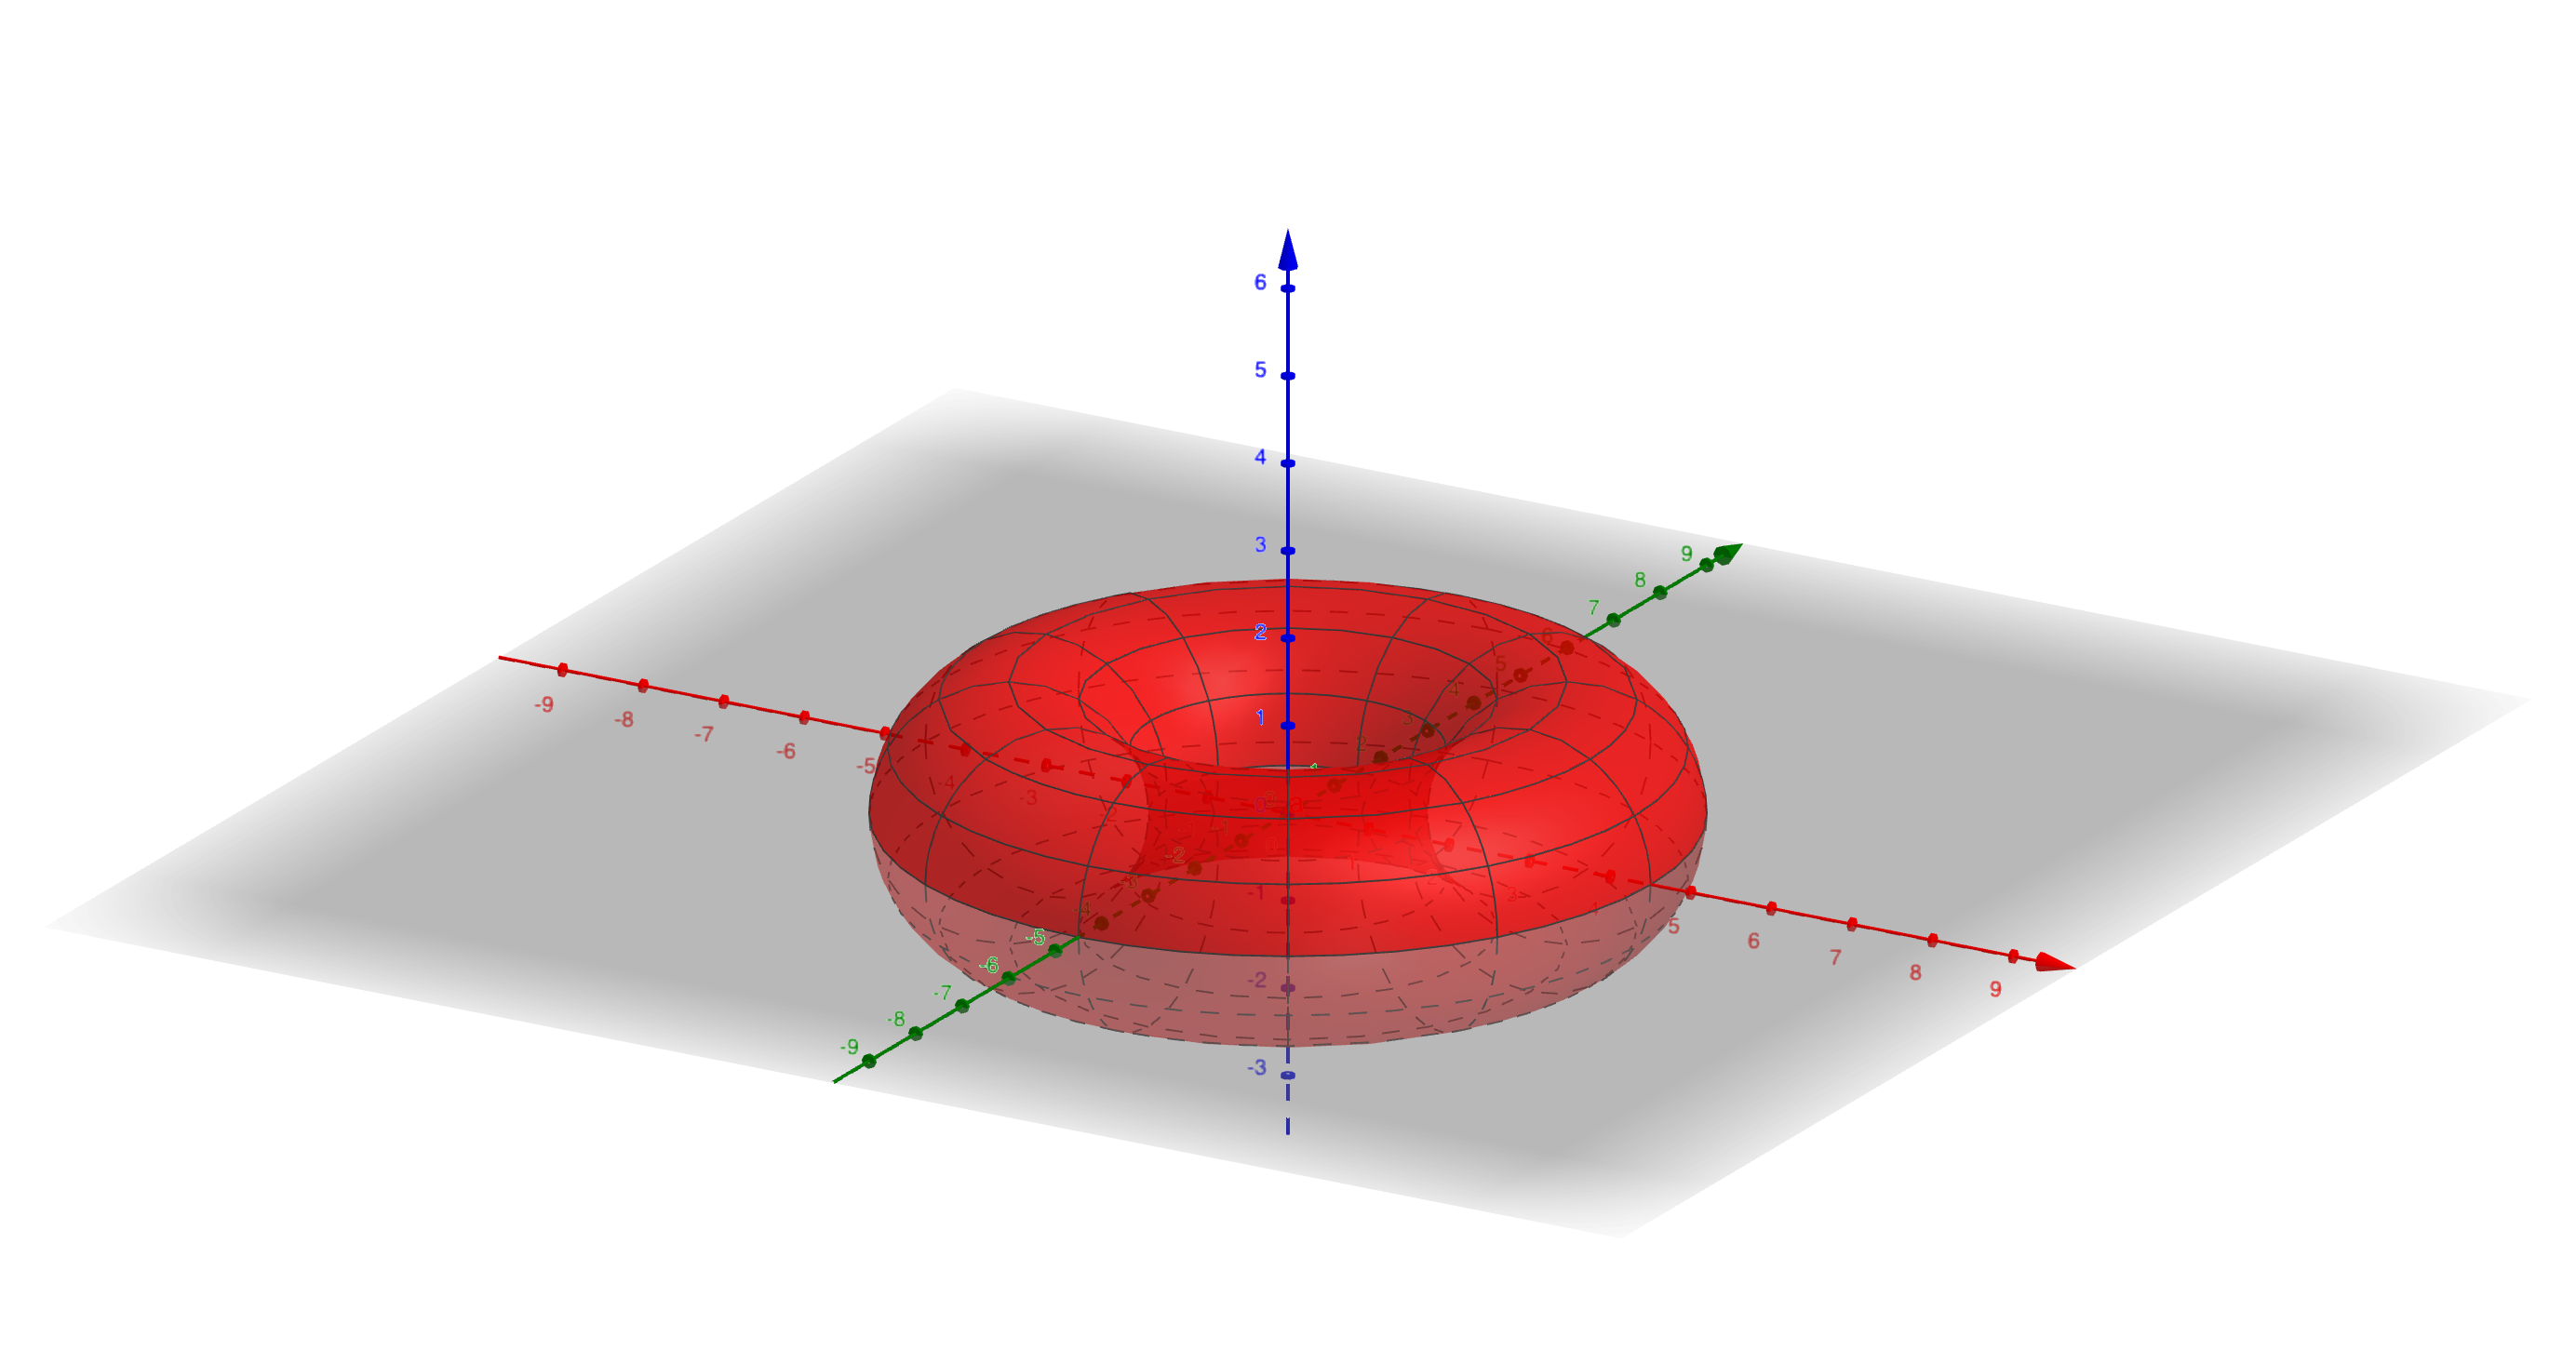
\includegraphics[width=.4\textwidth]{Figures_Part_6/torus.png}
                \end{figure}
                \end{ex}
                
                
                We have given ourselves ways of understanding the scalar functions and curves, but still need to develop a manner to understand vector fields.  We will not only need to understand vector fields in their own right, but we will need them in order to investigate how the scalar fields change from point to point.  Roughly speaking, the ``derivative" of a scalar field will be a vector field.
                
                 \section{Approximation and the Tangent Space}
                                        Sometimes it is helpful to know what a surface looks like up close.  In this case, the surface is best approximated by a plane.  This is analogous to how you can approximate functions of a single variable by a line.
                                        
                                        \begin{exercise}
                                        Compute the tangent line to $f(x)=2x^2+5$ at the point $x_0=3$.
                                        \end{exercise}
                                        
                                        \subsubsection{Equation for a Plane}
                                        
                                        We haven't worked much with planes in space yet, but we have seen surfaces.  In some sense, planes are the easiest surfaces.  They are, after all, linear objects.
                                        
                                        \begin{ex}{Plane and Normal}{plane_normal}
                                        The equation for a plane is given by
                                        \[
                                        ax+by+cz+ d = 0.
                                        \]
                                        Notice that this is a linear equation.
                                        
                                        Then the \emph{normal vector} to the plane is given by 
                                        \[
                                        \mathbf{n} = \begin{bmatrix} a \\ b \\ c\end{bmatrix}.
                                        \]
                                        We can see a diagram of this here.
                                        \begin{figure}[H]
                                            \centering
                                            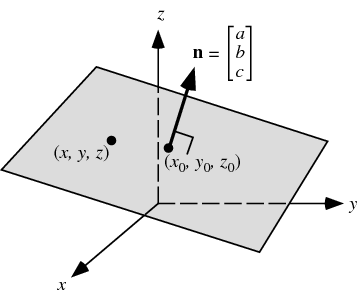
\includegraphics[width=.4\textwidth]{Figures_Part_6/plane_n.png}
                                        \end{figure}
                                        \end{ex}
                                        
                                        Now, if we are given a surface (defined as a level surface or as the graph of a function), we can compute an approximation at a point called the \emph{tangent plane}.
                                        
                                        \begin{ex}{Tangent Plane to Paraboloid}
                                        Consider the function 
                                        \[
                                        f(x,y)=-x^2-y^2.
                                        \]
                                        Then the graph of the function is given by plotting the points
                                        \[
                                        (x,y,f(x,y)).
                                        \]
                                        We compute the tangent plane by computing partial derivatives. We take
                                        \begin{align*}
                                        \frac{\partial f}{\partial x} &= -2x\\    
                                        \frac{\partial f}{\partial y} &= -2y.
                                        \end{align*}
                                        Then the equation for a tangent plane at the point $(x_0,y_0,f(x_0,y_0))$ is given by
                                        \[
                                        z-f(x_0,y_0)=\partialx (x-x_0)+\partialy (y-y_0).
                                        \]
                                        So in our case, we have
                                        \[
                                        z-(-x_0^2-y_0^2)=-2x_0(x-x_0)-2y_0(y-y_0).
                                        \]
                                        Pictorially, it looks as follows (letting $p=(x_0,y_0,f(x_0,y_0))$):
                                        \begin{figure}[H]
                                            \centering
                                            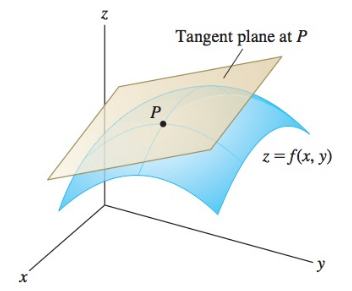
\includegraphics[width=.4\textwidth]{Figures_Part_6/tangent-planes-1.png}
                                        \end{figure}
                                                
                                        \end{ex}
                                        
                                        \begin{ex}{Tangent Vectors}{tangent_vectors}
                                        Another way to understand this is to compute the \emph{tangent vectors} at a point. Take the same function $f(x,y)=-x^2-y^2$ and compute
                                        \begin{align*}
                                            \frac{\partial}{\partial x}\begin{bmatrix} x \\ y \\ f(x,y)\end{bmatrix} &= \begin{bmatrix} 1\\ 0 \\ -2x\end{bmatrix}\\
                                            \frac{\partial}{\partial y}\begin{bmatrix} x \\ y \\ f(x,y)\end{bmatrix} &= \begin{bmatrix} 0\\ 1 \\ -2y\end{bmatrix}.
                                        \end{align*}
                                        Then take the cross product of these two vectors to get the normal vector to the tangent plane
                                        \[
                                        \begin{bmatrix} 1 \\ 0 \\-2x\end{bmatrix} \times \begin{bmatrix} 0 \\ 1 \\ -2y\end{bmatrix} = \begin{bmatrix} 2x \\ 2y \\ 1\end{bmatrix}.
                                        \]
                                        Pick a point $(x_0,y_0)$ and the normal to tangent plane is given by
                                        \[
                                        \mathbf{n}=\begin{bmatrix} 2x_0 \\ 2y_0 \\ 1 \end{bmatrix}.
                                        \]
                                        Which leads us to the following equation of a plane (but not exactly the tangent plane)
                                        \[
                                        2x_0 x + 2y_0y+z=0.
                                        \]
                                        This plane is parallel to the tangent plane and is often a nicer tool.
                                        \end{ex}
                                        
                                        \begin{exercise}
                                        Take the two equations for the planes above and simplify each to having a zero right hand side.  Then subtract each of these equations from each other and see what the difference is.
                                        \end{exercise}
                